% CVPR revision of the AAAI manuscript, with reviewer-driven corrections and experiments.
% See REVISION_STATUS.md before submission.
\documentclass[10pt,twocolumn,letterpaper]{article}
\usepackage[review]{cvpr}
% TeX Live 2019 compatibility: evaluate arithmetic dimensions in the uploaded
% template's shipout coordinates; otherwise literal "-12pt" appears in header.
% No change to the intended dimensions or to cvpr.sty.
\makeatletter
\renewcommand{\LenToUnit}[1]{\strip@pt\dimexpr#1\relax}
\makeatother
\usepackage{algorithm}
\usepackage{algorithmic}
\newcommand{\sg}{\operatorname{sg}}
\newcommand{\rms}{\operatorname{RMS}}
\newcommand{\normr}{\operatorname{RMSNorm}}
\graphicspath{{figures/}}

% Visible result slots in this working draft. Fill each slot before submission.
\newcommand{\pendingcell}{\textit{TBD}}
\newcommand{\pendingexperiment}[2]{%
  \par\smallskip\noindent
  \fbox{\parbox{\dimexpr\linewidth-2\fboxsep-2\fboxrule\relax}{%
    \textbf{#1 (pending).} #2}}%
  \par\smallskip
}

\definecolor{cvprblue}{rgb}{0.21,0.49,0.74}
\usepackage[pagebackref,breaklinks,colorlinks,allcolors=cvprblue]{hyperref}
\def\confName{CVPR}
\def\confYear{2027}
\title{Test-Time Score Distillation: Mask-Free Semantic Style Editing with Reverse-Process Regularization}
\author{Anonymous Authors}
\begin{document}
\maketitle
\begin{abstract}
A style reference carries not only artistic appearance but also objects and
composition, making it difficult to transfer its medium to a new subject.
We cast training-free style transfer as test-time score distillation (TSD)
on a frozen rectified-flow text-to-image transformer. At inference, we
optimize only the current latent using the model's image-conditioned
CFG-augmentation contrast, computed from velocity predictions with and
without a style reference at the identical latent state and noise level.
The corresponding score direction is RMS-normalized to construct a
detached clean-state target, and latent updates are interleaved with
frozen reverse sampling, which provides reverse-process regularization. TSD trains no weights and
requires no attention-feature modification, additional adapter, fake-score
network, or generator. Adjusting the reverse sampling and latent
intervention schedules supports both semantic style editing with greater
composition preservation and global style transfer with freer composition.
Experiments across artistic media and target prompts show stronger
reference style matching than the backbone's native image-and-text editing
and direct reference guidance, while retaining recognizable target subjects.
\end{abstract}

\section{Introduction}
\label{sec:intro}

Style transfer on a frozen generator is treated as one task, but
users want two. Given a content prompt and a reference image, a frozen
text-to-image transformer can render the prompt's subject ``in the style of''
the reference. In practice two very different outcomes are desirable and are
conflated under one name. In one, an artist wants the reference's
\emph{scene} preserved, including its composition and arrangement, with only the
subject re-imagined in the reference's medium. This is \emph{Semantic Style
Editing}. In the other, the artist wants only the reference's \emph{look},
including its medium, texture, and palette, carried onto a freshly composed
scene, with the reference's specific layout thrown away. This is
\emph{Global Style Transfer}. The desired amount of reference-layout retention therefore depends on
the creative task.

These two outcomes motivate a common \emph{style-locality} axis.
Style locality describes how much reference layout is retained. Greater
retention supports semantic editing, while freer composition supports global
transfer. We assess this axis separately from reference-medium fidelity and
target-subject alignment, so replacing the reference subject remains an
explicit requirement in either task.

We drive this axis with one frozen-model operator. Distribution-matching
distillation separates CFG augmentation, which strengthens conditioning,
from distribution matching with a learned fake-score estimate
\citep{yin2024dmd,liu2025decoupled}. Our setting differs: we optimize a
single inference-time latent while retaining the frozen reverse process.
The native reference-conditioning contrast supplies the style direction,
and ordinary reverse steps continue the model's denoising trajectory
between latent interventions. We call this procedure \textbf{Test-Time
Score Distillation (TSD)} and its alternation \emph{reverse-process
regularization}.

TSD evaluates reference-conditioned and reference-free velocities at the
same latent state, noise level, and target text. We convert their difference
to a score direction, RMS-normalize it, and construct a detached clean-state
target for latent optimization. The target is rebuilt after each inner
update. All network weights remain frozen, with no learned style adapter,
auxiliary fake-score network, or spatial mask. Sampling resolution and
intervention settings jointly determine the style-locality operating point.

\paragraph{Contributions.}
\begin{enumerate}
\item \textbf{A common task formulation.} Semantic Style Editing and Global
Style Transfer are two goals on a style-locality axis. We serve both with
one operator and study their sampling and latent-intervention settings.
\item \textbf{Test-time score distillation with reverse-process
regularization.} We turn the frozen model's same-state reference contrast
into an RMS-normalized pseudo-target for latent optimization, interleaved
with its native reverse trajectory.
\item \textbf{A separable-axis evaluation protocol.} We evaluate style
fidelity with CSD, subject fidelity with CLIP-T, and composition transfer
with reference-layout similarity, interpreting all three together.
\item \textbf{Native-editor and dedicated-method comparisons.} We retain
the initial 40-reference study and extend it with multiple prompts, a strong
same-backbone reference-CFG control, and dedicated transfer methods. The joint readouts expose how guidance and intervention settings affect
style, subject, and composition.
\end{enumerate}


\section{Related Work}
\label{sec:related}

\paragraph{Distillation and test-time score guidance.}
Distribution-matching distillation matches a student generator to a teacher
through teacher and fake-score estimates, with later variants improving the
objective and separating distribution matching from CFG augmentation
\citep{yin2024dmd,yin2024dmd2,liu2025decoupled}. This decomposition connects
to diffusion and score models' noise-conditional vector fields
\citep{ho2020ddpm,song2021sde}. Conditional contrasts appear in classifier
guidance, classifier-free guidance, score distillation, and text-guided editing
\citep{dhariwal2021diffusion,ho2022cfg,poole2023dreamfusion,hertz2023dds,
nam2024cds,chinchuthakun2025lusd}.
Other test-time methods steer frozen samplers with external losses, perturbed
attention, or annealed conditions
\citep{bansal2023universal,ahn2024pag,hong2024seg,sadat2024cads}. TSD applies the reference-conditioned augmentation direction to one
test-time sample. It optimizes the current latent and interleaves these
updates with the frozen reverse trajectory.

\paragraph{Reference-conditioned style transfer and frozen-model editing.}
Classical style transfer matches feature statistics
\citep{gatys2016style,huang2017adain}. Diffusion methods extend this idea
through exemplar conditioning, learned style interfaces, attention sharing,
or sampling-time transport
\citep{yang2023paint,sohn2023styledrop,ye2023ipadapter,hertz2024stylealigned,
chung2024styleinjection,deng2024zstar,wang2024instantstyle,xu2025stylessp,
he2025semantix,rout2025rbmodulation}. Related editing systems control cross-attention or reuse
frozen diffusion features \citep{hertz2023prompt,tumanyan2023plugplay}, while
rectified-flow methods develop inversion and direct trajectory editing
\citep{rout2025rfinversion,kulikov2025flowedit}. TSD belongs to the
optimization-based, training-free-of-weights family, but its signal is the
native same-state reference-conditioning contrast rather than replaced
attention features, a trained adapter, or an explicit mask. We evaluate medium, palette, and texture transfer together with reference-layout
retention, without requiring exact correspondence of individual motifs.

\paragraph{Dedicated transfer systems and latent optimization.}
Attention Distillation is a close optimization-based comparison: it updates
the sampling latent using an attention-derived reference loss
\citep{zhou2025attentiondistillation}. StyleShot uses a style-aware image
encoder \citep{gao2024styleshot}, CSGO learns content--style composition
\citep{xing2024csgo}, and USO supports style and subject customization
\citep{wu2025uso}. TSD uses the native reference-conditioned velocity
contrast as its supervision. Our comparisons distinguish reference-plus-text
generation from methods that additionally require a content image.


\section{Method}
\label{sec:method}
Figure~\ref{fig:method} summarizes the operator derived in this section as
an alternating cycle of task-direction distillation, latent optimization,
and frozen-prior regularization. The reference contrast supplies the task
direction, an RMS-normalized pseudo-target defines the latent objective,
and the reverse process advances the sample between interventions.

\subsection{Task and native reference conditioning}
\label{sec:conditioning}
Let $r$ denote the reference image and $c$ the full target instruction,
including the requested subject and transfer instruction. We consider two
objectives. \emph{Semantic style editing} seeks the requested subject in the
reference medium with substantial reference-layout retention.
\emph{Global style transfer} seeks the medium in an independently composed
image. In both cases, the target text specifies the output subject, while the
reference supplies the medium and, to a task-dependent degree, layout.

The frozen transformer predicts a velocity at latent $z_\sigma$ and noise
level $\sigma$. We query its native conditioning interface twice:
\begin{equation}
\begin{aligned}
v_r&=v_\theta(z_\sigma,\sigma,c,r),\\
v_b&=v_\theta(z_\sigma,\sigma,c,\varnothing).
\end{aligned}
\label{eq:branches}
\end{equation}
In the Klein implementation, the frozen VAE encodes the reference into
auxiliary image tokens. The transformer receives these tokens together
with the current noisy-image tokens and target-text representation.
Image-position identifiers distinguish the reference tokens from the
output tokens. The reference-free branch omits the auxiliary image tokens.
Text, latent state, noise level, and output geometry are shared between
the two queries, so their difference measures the response to adding the
reference condition.

\begin{figure*}[t]
\centering
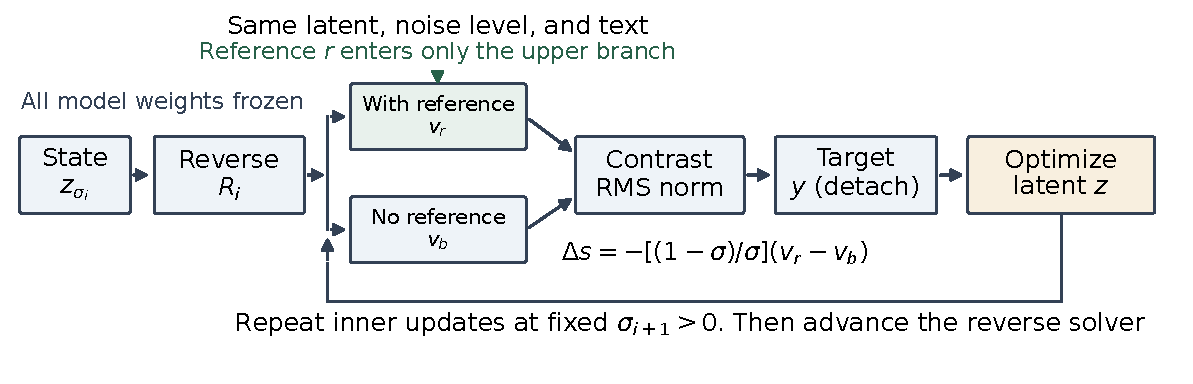
\includegraphics[width=\textwidth]{method.pdf}

\caption{TSD inference. The frozen reverse step reaches
$\sigma_{i+1}$, where paired reference-conditioned and reference-free
predictions define an RMS-normalized score direction. A detached target
then guides inner latent optimization at the reached noise level.
The cycle repeats with all network weights frozen.}
\label{fig:method}
\end{figure*}

\subsection{From velocity contrast to a score target}
\label{sec:target}
We express the native conditioning contrast in score space using the
rectified-flow interpolation
$z_\sigma=(1-\sigma)x_0+\sigma\epsilon$, with Gaussian $\epsilon$ and
velocity convention $v=\epsilon-x_0$. The clean estimate and score satisfy
\begin{align}
\hat x_0&=z_\sigma-\sigma v,\label{eq:clean}\\
s_\theta&=-\frac{z_\sigma+(1-\sigma)v_\theta}{\sigma}.
\label{eq:score}
\end{align}
Equation~\ref{eq:score} follows from the Gaussian-noise score identity with
the conditional-mean velocity. A learned field approximates that quantity
\citep{lipman2023flow,liu2023rectified}. The shared state cancels when the
two conditions in Eq.~\ref{eq:branches} are contrasted:
\begin{equation}
\Delta s_\sigma=s_r-s_b
=-\frac{1-\sigma}{\sigma}(v_r-v_b).
\label{eq:sign}
\end{equation}
The factor $-(1-\sigma)/\sigma$ fixes the orientation of the score
direction under this velocity convention. We clamp the denominator near
zero and apply optimization only at positive noise levels.

RMS normalization makes the target offset insensitive to most changes in
field magnitude across noise levels. For a positive multiplier $a$ and
normalization floor $\varepsilon_g$, define
\begin{equation}
g=a\Delta s_\sigma,\qquad
 d=\frac{g}{\max\!\left(\sqrt{N^{-1}\sum_{j=1}^N g_j^2},\varepsilon_g\right)},
\label{eq:normalization}
\end{equation}
where $N$ counts latent elements per sample. Away from the numerical
floor, the positive multiplier $a$ cancels under normalization. The
resulting direction has unit RMS, giving the target offset a consistent
scale across noise levels.

\subsection{RMS-normalized pseudo-target distillation}
\label{sec:optimization}
The pseudo-target supplies a first-order optimization signal without
backpropagating through the frozen transformer. With $\sg$ denoting
stop-gradient, each inner iteration forms
\begin{align}
\hat x_0(z)&=z-\sigma\sg(v_b),\\
y&=\sg\!\left(\hat x_0(z)+\eta d\right),\\
L_{\rm p}&=\frac{1}{2N}\sum_{j=1}^N(\hat x_{0,j}(z)-y_j)^2,
\label{eq:pseudoloss}
\end{align}
where $\eta$ sets the normalized target offset. Both teacher predictions
used to construct $d$ are detached and recomputed at the current inner-loop
state. The target is rebuilt before each loss evaluation, then treated as a
constant during differentiation.

Detaching the velocity makes the clean-estimate Jacobian the identity in
this branch. Thus
\begin{equation}
\frac{\partial\hat x_0}{\partial z}=I,
\qquad \nabla_z L_{\rm p}=-\frac{\eta}{N}d.
\label{eq:gradient}
\end{equation}
The mean reduction contributes $1/N$. For SGD with learning rate $\ell$,
the displacement is $\ell\eta d/N$. We use AdamW, whose moment estimates
and numerical stabilization determine the displacement from this gradient.
Thus $\eta$ controls the target offset and $\ell$ controls the optimizer
step. The supplementary derivation gives both update expressions.

The evaluated TSD operator uses $L_{\rm p}$ as its latent objective.
We initialize AdamW with zero weight decay at each outer intervention and
retain its moments across the inner iterations at that node. Recomputing
the target after every update keeps the reference contrast evaluated at
the current state. No warm-start or output AdaIN transformation is used.

\paragraph{Why a directional target?}
The target uses the direction of the reference contrast rather than a loss
that forces the two predictions to agree. Minimizing
$\frac12\|\Delta s(z)\|^2$ would differentiate the contrast itself and
produce $J_{\Delta s}(z)^\top\Delta s(z)$. Our detached target instead gives
the first-order direction in Eq.~\ref{eq:gradient}, without differentiating
the teacher. Normalization keeps the target offset informative even when
the contrast magnitude changes along the trajectory. Rebuilding the target
after each update lets successive interventions follow the reference
response at the edited state.

\subsection{Reverse-process regularization and style locality}
\label{sec:schedule}
The reference contrast provides a task direction, while the reverse field
provides the generative dynamics. This separation is motivated by the
CFG-augmentation and distribution-matching components of decoupled DMD
\citep{liu2025decoupled}. Their roles occur in different optimization
problems: DMD updates generator weights using a learned estimate of the
student distribution, whereas TSD updates one latent inside an existing
multi-step sampler. We retain that sampler as the regularizing component
of the inference procedure. No learned student-distribution estimate is
needed to define or execute the TSD operator.

We implement reverse-process regularization by alternating reference-directed
latent optimization with the frozen model's text-conditioned reverse steps.
The reverse solver advances the state before a guidance intervention. Let
$\sigma_0>\cdots>\sigma_M=0$ be its actual noise nodes and $R_i$ its reverse
update. From $z_{\sigma_i}$, we first obtain
$z^{(0)}_{\sigma_{i+1}}=R_i(z_{\sigma_i})$. If the reached positive node
belongs to the intervention set $\mathcal G$, we apply $K_i$ latent
optimization steps there. At other nodes we retain the solver output.
Algorithm~\ref{alg:tsd} specifies this order. The final reverse step has no
subsequent inner optimization.

\begin{algorithm}[t]
\caption{TSD inference}
\label{alg:tsd}
\begin{algorithmic}[1]
\REQUIRE Frozen $v_\theta$, instruction $c$, reference $r$, solver nodes,
interventions $\mathcal G$, inner counts $K_i$, $\eta$, optimizer rate $\ell$
\STATE Initialize Gaussian latent $z_{\sigma_0}$
\FOR{$i=0,\ldots,M-1$}
\STATE $z\gets R_i(z_{\sigma_i})$ at $\sigma_{i+1}$
\IF{$\sigma_{i+1}\in\mathcal G$ and $\sigma_{i+1}>0$}
\STATE Initialize latent optimizer at $z$
\FOR{$k=1,\ldots,K_i$}
\STATE Evaluate detached $v_r,v_b$ at the same $(z,\sigma_{i+1},c)$
\STATE Construct $d$, $y$, and $L_{\rm p}$ using Eqs.~\ref{eq:normalization}--\ref{eq:pseudoloss}
\STATE Update only $z$ using $\nabla_z L_{\rm p}$
\ENDFOR
\ENDIF
\STATE $z_{\sigma_{i+1}}\gets z$
\ENDFOR
\STATE Decode $z_{\sigma_M}$
\end{algorithmic}
\end{algorithm}

\paragraph{Style locality and working points.}
The solver nodes determine where reverse sampling evaluates the model,
while $\mathcal G$, $K_i$, $\eta$, and $\ell$ determine the latent
interventions. We use their joint settings to obtain different degrees of
style strength and reference-layout retention. The retained configurations
use 25 reverse intervals with two inner updates and $\eta=.05$, or eight
intervals with five inner updates and $\eta=.12$. Both use learning rate
$.01$. Inner updates occur after eligible positive reverse nodes.
For controlled comparisons of discretization, we also insert shared
positive nodes and assign the same inner count at each node. This separates
solver resolution from intervention location and count.

\subsection{Relationship to CFG and computational cost}
\label{sec:controls}
Text guidance and reference guidance act on different conditions.
Let $v_u^\beta$ denote text CFG applied with image condition $u$, using
$v_{\rm uncond}+\beta(v_{\rm cond}-v_{\rm uncond})$ within that branch.
Direct reference guidance advances the reverse solver with
\begin{equation}
 v_{\rm refCFG}^{\beta}=v_b^{\beta}
       +\gamma(v_r^{\beta}-v_b^{\beta}).
\label{eq:referencecfg}
\end{equation}
Both image conditions use the same text scale $\beta$. In the retained TSD
settings, the reverse step uses the reference-free, text-guided velocity
$v_b^\beta$. Reference information enters through the inner score-contrast
target at fixed instruction $c$. The sampler text scale $\beta$, direct
reference scale $\gamma$, and score multiplier $a$ are recorded separately.

\paragraph{Computation.}
Each inner iteration evaluates the two frozen teacher branches and
backpropagates through the detached-target loss to the latent. The
transformer is evaluated under stop-gradient, so its activations need not
be retained for latent differentiation. With
$U=\sum_i K_i$ inner iterations, an uncached implementation adds $2U$
teacher evaluations to reverse sampling. Prediction sharing can reduce
this count. The cost analysis records model calls and latent backward calls. The final
latency and memory comparison will use common hardware with explicit
text-guidance and offload settings.

\section{Experiments}
\label{sec:experiments}
We evaluate TSD along the three axes introduced above: reference medium,
requested subject, and reference-layout retention. The initial study tests
both task regimes against the native editor on 40 references. An expanded
study adds multiple prompts, dedicated style-transfer methods, and stronger
same-backbone guidance controls. We then examine how latent interventions
change the balance between style and subject fidelity.

\subsection{Experimental setup}
\label{sec:setup}
\paragraph{Initial and expanded studies.}
The initial study uses 40 style references with the prompt ``a panda eating
bamboo'' and seed 65. It compares the original semantic and global TSD
configurations with native editing instructions that respectively request
reference-layout retention and a new composition. We retain its stored
measurements as a distinct study. The expanded study uses newly generated
outputs with recorded configurations and input/output hashes.

The new reference collection contains 48 public Krea-generated images across
eight medium categories. We selected references for medium clarity, visual
quality, and diversity before inspecting generated outputs. Each category
contributes one development and five test references, giving an 8/40 split.
Every method receives the same RGB $512\times512$ reference, obtained by
aspect-preserving resizing and center cropping of the public 1024-pixel
source version. Six fixed prompts request a panda, castle, cat, sunflower
field, fisherman portrait, and lighthouse. Source identifiers, transforms,
and image hashes are provided in the supplementary records. The completed
expanded comparison uses the eight development references and seed 64.
The 40 disjoint references are reserved for the multi-seed test protocol
in Sec.~\ref{sec:expanded}.

\paragraph{Comparison methods.}
The common task supplies a style reference and target text. TSD and
reference CFG share the frozen Klein-9B-base backbone, text CFG 4, and the
same transfer instruction. The reference-CFG baseline is chosen from a
development sweep of guidance strengths and sampling budgets. Its retained
setting uses 72 intervals and reference scale $\gamma=5$.
Attention Distillation (AD) uses SD1.5 with 50 steps, two inner updates,
learning rate .015, text CFG 7.5, and AdaIN
\citep{zhou2025attentiondistillation}. USO uses its style-only interface
with FLUX.1-dev, pretrained rank-128 adapters and SigLIP features, 25 steps,
and guidance 4 \citep{wu2025uso}. USO stores weights in FP8 with bf16
computation. Backbones, pretrained adapters, and precision are recorded
alongside the method settings. StyleShot uses its pretrained SD1.5
style encoder and adapter with style scale 1, text CFG 7.5, and the official
float32 pipeline \citep{gao2024styleshot}. Its nominal 50-step PNDM schedule
performs 51 UNet evaluations. InstantStyle uses the official style-block
IP-Adapter interface on SDXL, with 30 Euler steps, text CFG 5, style scale
1, and float16 inference \citep{wang2024instantstyle}. Its image condition
enters the designated style block. Quality and negative prompts follow
the official example and are recorded in the supplement.

\paragraph{Metrics and paired analysis.}
We report CSD reference--output similarity for style
\citep{somepalli2024csd}, CLIP ViT-B/32 image--text similarity to the literal
content request \citep{radford2021clip}, and DINOv2 ViT-B/14 reference-layout
similarity \citep{oquab2024dinov2}. For normalized patch features $P_x$,
let $q_x=\operatorname{vec}_{\rm off}(P_xP_x^\top)$. The layout measure is
\begin{equation}
\Lambda(x,r)=\operatorname{corr}(q_x,q_r).
\label{eq:layout}
\end{equation}
Higher $\Lambda$ indicates more similar spatial self-similarity structure,
which can be useful for semantic editing. Both geometry and shared
semantics can affect this readout. We compute method differences on matched
reference/prompt/seed cells and bootstrap reference groups with all their
repeated observations together, using 10,000 resamples.

\subsection{Full benchmark against the frozen model's native edit}
\label{sec:initialresults}
The same frozen model's native image-and-text editing path provides the
initial baseline. In TSD, the reference enters the score-contrast objective
while the reverse solver itself uses the reference-free branch. Setting the
contrast to zero therefore gives text-only sampling, rather than native
image editing. The native keep-layout and new-layout instructions are
separate reference-conditioned comparisons.

The initial study tests whether one operator can strengthen the reference
medium under both composition objectives. Table~\ref{tab:benchmark} retains
the original 160 measurements, with sample SD across the 40 references.
The table summarizes the stored measurements from the initial study.
Its complete per-reference records appear in the supplement.

\begin{table}[t]
\centering\small
\caption{Initial 40-reference study, one content prompt and seed 65.
Values are mean $\pm$ sample SD across references. S/G are the original
semantic/global configurations. Layout measures retention of reference
structure, whose desired level depends on the task.}
\label{tab:benchmark}
\resizebox{\columnwidth}{!}{\begin{tabular}{lccc}
\toprule
Method & CSD $\uparrow$ & CLIP-T $\uparrow$ & Layout \\
\midrule
TSD-S (semantic) & 0.719 $\pm$ 0.079 & 0.295 $\pm$ 0.031 & 0.572 $\pm$ 0.148 \\
TSD-G (global) & 0.615 $\pm$ 0.096 & 0.304 $\pm$ 0.027 & 0.414 $\pm$ 0.109 \\
Native keep-layout & 0.267 $\pm$ 0.165 & 0.319 $\pm$ 0.012 & 0.317 $\pm$ 0.073 \\
Native new-layout & 0.247 $\pm$ 0.157 & 0.315 $\pm$ 0.011 & 0.299 $\pm$ 0.065 \\
\bottomrule
\end{tabular}
}
\end{table}

TSD-S increases mean CSD from .267 to .719 relative to native keep-layout
editing, and TSD-G increases it from .247 to .615 relative to native
new-layout editing. Every reference has a positive paired CSD difference
in both comparisons. CLIP-T decreases from .319 to .295 and from .315 to
.304, respectively. The two TSD configurations also differ in layout
retention: .572 for S and .414 for G. Thus the original study supports two
useful operating regimes, with stronger reference matching accompanied by
different amounts of reference structure.

CLIP-T is read against the literal content request, separately from the
style-transfer instruction. The earlier five-reference, four-additional-prompt
study is retained in the supplement using its stored prompt-level summaries.
The new multi-prompt comparison below has its own inputs and measurements.

The style increase must be interpreted together with composition. Against
each output's paired native baseline, only 1/40 semantic and 3/40 global
outputs have no greater layout similarity. The full-set CSD gains therefore
do not by themselves establish a style advantage at matched layout. The
expanded study below evaluates this condition explicitly and includes a
swept reference-guidance control.

\subsection{Expanded reference-plus-text comparison}
\label{sec:results}
We select TSD settings and direct-reference controls on a 16-cell grid of
four references, two prompts, and two seeds. The resulting 25-configuration
study contains 400 outputs. We then compare the retained settings, AD, USO,
StyleShot, and InstantStyle on all eight development references and six prompts at seed
64, giving 48 paired inputs per method. Table~\ref{tab:coverage} reports all
336 outputs in this comparison. The supplementary material gives the full
configuration study, including exact reused cells.

\begin{table}[t]
\centering\small
\caption{Development coverage on eight references, six prompts, and seed
64 (48 outputs per row). Layout measures reference-layout retention.
Backbones and precision are specified in the setup.}
\label{tab:coverage}
\resizebox{\columnwidth}{!}{\begin{tabular}{lrrr}
\toprule
Method & CSD $\uparrow$ & CLIP-T $\uparrow$ & Layout \\
\midrule
Reference CFG, 72/$\gamma=5$ & 0.3190 & 0.3005 & 0.3118 \\
AD (SD1.5) & 0.7069 & 0.2692 & 0.3224 \\
USO (FLUX.1, FP8) & 0.4117 & 0.3178 & 0.2953 \\
StyleShot (SD1.5) & 0.5042 & 0.2840 & 0.2703 \\
InstantStyle (SDXL) & 0.4947 & 0.2616 & 0.2900 \\
TSD, 8/K5 & 0.4291 & 0.3078 & 0.3101 \\
TSD, 25/K2 & 0.5751 & 0.2982 & 0.3503 \\
\bottomrule
\end{tabular}
}
\end{table}

\begin{figure*}[t]
\centering
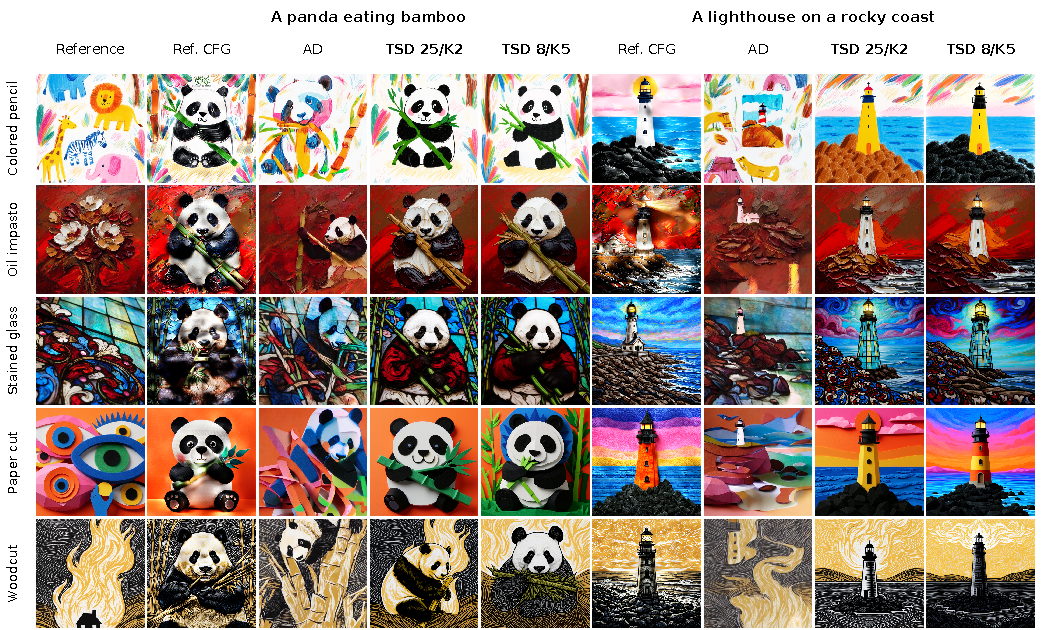
\includegraphics[width=\textwidth]{two_prompt_comparison.pdf}
\caption{Reference-guided generation across two content prompts and five media.
Each row shares a reference. Each prompt block compares reference CFG,
Attention Distillation, and two TSD settings on the same input and seed 64.
TSD preserves characteristic color, material, and surface patterns across
the two subjects. The 25/K2 and 8/K5 settings change the strength and spatial
expression of the reference signal. These outputs belong to the expanded
development comparison in Table~\ref{tab:coverage}.}
\label{fig:twoprompt}
\end{figure*}

Both TSD settings strengthen style matching over the selected reference-CFG
baseline. TSD8/K5 raises mean CSD from .3190 to .4291 and CLIP-T from .3005
to .3078. The paired differences are .1101 for CSD (reference-group 95\%
bootstrap interval $[.0720,.1463]$) and .0073 for CLIP-T
($[.0004,.0157]$). Its mean layout similarity is .3101, compared with .3118
for the direct control. TSD25/K2 further increases CSD to .5751, with
CLIP-T .2982 and layout similarity .3503. Its paired CSD increase over
reference CFG is .2561 ($[.2178,.2940]$).

The dedicated methods place these settings in a broader style--subject
comparison. Relative to AD, TSD25/K2 has higher CLIP-T by .0291
($[.0233,.0354]$) and lower CSD by .1319 ($[.0559,.2049]$ for AD minus TSD).
Relative to USO, it has higher CSD by .1633 ($[.0876,.2506]$) and lower
CLIP-T by .0195 ($[.0149,.0249]$ for USO minus TSD). TSD8/K5 favors subject
alignment within our two settings, while TSD25/K2 strengthens the style
signal. StyleShot obtains CSD .5042 and CLIP-T .2840, compared with .5751 and
.2982 for TSD25/K2. InstantStyle obtains CSD .4947 and CLIP-T .2616. These development
comparisons use eight reference groups.

Figure~\ref{fig:twoprompt} shows how the reference signal appears in different
media and subjects. In stained glass, TSD carries colored panes and dark
outlines into both the panda and lighthouse. The paper-cut examples retain
layered shapes, while the oil-paint examples reproduce broad impasto strokes.
The two TSD settings also differ visibly in framing and surface treatment.
These examples complement the joint metric readout: medium transfer and
reference-layout retention are related properties, but neither is a
substitute for rendering the target subject.

\paragraph{Paired layout constraint.}
We also evaluate style differences on cells whose TSD output retains no
more layout than its corresponding baseline output:
\begin{equation}
\mathcal I=\{i:\Lambda(x_i^{\rm TSD},r_i)
\leq\Lambda(x_i^{\rm baseline},r_i)\}.
\label{eq:pairedconstraint}
\end{equation}
Against reference CFG, TSD8/K5 satisfies this condition on 22/48 cells.
Within this subset, its mean CSD and CLIP-T differences are .0867 and .0041.
TSD25/K2 satisfies the condition on 18/48 cells, with differences .2127
and $-.0045$. We report these descriptive subset results together with their
coverage and the complete-grid comparison.

\subsection{The style-locality axis and ablations}
\label{sec:interventioncontrols}
\paragraph{Why use a moderate update count?}
At a fixed 25-step solver, learning rate .01, and target offset .05,
K1/K2/K5 produce CSD .3726/.5555/.7302 and CLIP-T
.3109/.3110/.2796 on the same 16-cell search grid. K2 strengthens style
relative to K1 while retaining a similar subject score, and uses 146 DiT
forwards compared with 290 for K5. This motivates the retained 25/K2
setting. Reducing the K5 learning rate to .005 instead gives CSD .6288 and
CLIP-T .2986. Update count and learning rate therefore provide different
style--subject operating points.

\paragraph{Sampling and intervention location.}
The common-node controls insert $\{.8,.6,.4,.2\}$ and perform one update
at each positive node. This fixes guidance locations and counts across
nominal solver lengths. The dense configurations intervene at the original
positive solver nodes. We record actual intervals, optimizer choice,
update count, and displacement for each configuration. The complete search
also includes RMS-SGD and shorter reference-guidance controls. At the four
shared nodes, nominal 25-step and eight-step sampling yield CSD
.0386/.0315 and CLIP-T .3190/.3168, respectively. Both have much lower
style similarity than the dense interventions in this study. These
measurements show the importance of the intervention schedule alongside
solver resolution. This design
compares discretization with matched intervention locations. The dense
8/K5 and 25/K2 settings instead change several factors together and define
operating points rather than an isolated effect of reverse-step count.

\paragraph{Model calls and timing.}
TSD8/K5 and TSD25/K2 use 86/146 DiT forwards and 35/48 latent backward
calls respectively. The backward calls differentiate the detached-target
loss. Reference CFG uses 288 DiT forwards, AD uses 200 UNet forwards, and
USO uses 25 DiT forwards under their respective settings. StyleShot uses
51 UNet forwards. Calls from
different backbones describe different computations. A common-hardware
timing comparison is reserved below.
End-to-end timing includes reference/text encoding, sampling, latent
optimization, and output decoding. Model loading is measured separately,
and single- and two-GPU placements are grouped separately in cost records.

\pendingexperiment{Inference cost}{Complete the same-hardware comparison
of end-to-end latency, peak allocated memory, precision, and offload policy.
Separate single- and two-GPU placements and report model loading separately.
The measured model-call counts above remain part of the completed analysis.}

\subsection{Multi-seed comparison}
\label{sec:expanded}
The held-out protocol uses 40 disjoint test references, six target prompts,
and seeds 64/65/66, giving 720 reference/prompt/seed cells per configuration.
The first frozen matrix contains reference CFG, AD, USO, and two TSD
settings, or 3,600 outputs. A separately validated extension adds StyleShot,
InstantStyle, and CSGO on the same inputs. The final comparison thus reserves
six baselines and two TSD settings, with a planned total of 5,760 outputs.
Table~\ref{tab:heldoutpending} provides the result slots. No test result is
used to select the method settings.

\begin{table}[t]
\centering\small
\caption{Held-out comparison, results pending. Each row has a planned
720 cells on the same 40-reference, six-prompt, three-seed grid. TBD denotes
an unfilled result, including rows whose generation may already be complete.}
\label{tab:heldoutpending}
\begin{tabular}{lccc}
\toprule
Method & CSD $\uparrow$ & CLIP-T $\uparrow$ & Layout \\
\midrule
Reference CFG & \pendingcell & \pendingcell & \pendingcell \\
AD & \pendingcell & \pendingcell & \pendingcell \\
USO & \pendingcell & \pendingcell & \pendingcell \\
StyleShot & \pendingcell & \pendingcell & \pendingcell \\
InstantStyle & \pendingcell & \pendingcell & \pendingcell \\
CSGO & \pendingcell & \pendingcell & \pendingcell \\
\midrule
TSD 8/K5 & \pendingcell & \pendingcell & \pendingcell \\
TSD 25/K2 & \pendingcell & \pendingcell & \pendingcell \\
\bottomrule
\end{tabular}

\end{table}

\pendingexperiment{Held-out results}{Complete generation, metric evaluation,
and reference-group paired intervals for the original matrix and validated
baseline extension. Fill Table~\ref{tab:heldoutpending}, followed by the
paired layout-constrained analysis and per-medium comparison.}

\subsection{Perceptual evaluation}
\label{sec:human}
The planned blinded study pairs TSD25/K2 with each of the six baselines on
40 fixed reference/prompt/seed cases. Each pair is assigned three independent
human judgments. The target is 240 pairs and 720 judgments, with separate
questions on style, subject, and overall preference. The displayed method
names are hidden and left/right positions are randomized. The supplementary
protocol specifies sampling and uncertainty estimation.

\pendingexperiment{Human preferences}{Collect the planned judgments and
report actual participant and response counts, wins, ties, unavailable
responses, and reference/rater-aware uncertainty. Overall preference is the
primary readout. No human preference result is available in this draft.}

\section{Discussion}
\label{sec:limitations}
TSD makes the frozen model's response to a reference an explicit objective
for the image latent. The reference signal and reverse sampling share one
model, and the intervention schedule provides different balances of style
strength, subject alignment, and layout retention. These properties make
TSD applicable to both composition-preserving semantic editing and freer
style-conditioned generation through a common operator.

The scope of the transfer follows the model's native reference
representation. A reference can convey object identity and layout as well
as material and texture, so the desired operating point depends on the
creative task. The current collection contains synthetic references, and
extending the evaluation to photographed materials and human-made artworks
would broaden the assessed range. Repeated teacher evaluations also make
inference cost an important design consideration. Prediction reuse and
adaptive intervention schedules are promising directions for reducing it.

\section{Conclusion}
\label{sec:conclusion}
Training-free style transfer on a frozen transformer serves Semantic Style
Editing and Global Style Transfer through a common style-locality framework.
TSD applies the native reference-conditioning score direction through
RMS-normalized detached targets for latent optimization. Interleaving those
updates with the frozen reverse trajectory provides reverse-process
regularization, without training a generator or auxiliary fake-score
network. The initial 40-style study and expanded comparisons show stronger
reference matching than native editing and direct reference guidance.
Sampling and intervention settings provide different balances of medium,
subject, and composition, with no mask or segmentation.

\section*{LLM Usage Statement}
OpenAI Codex assisted manuscript drafting and editing, mathematical and
code checks, protocol and experiment-script development, reference
curation, qualitative inspection, experiment management, and
figure/statistical-analysis code. The new reference images are
Krea-generated. Numerical results are computed from recorded executions.
The authors are responsible for verifying the text, references, data
provenance, and computations.
{\small\bibliographystyle{ieeenat_fullname}\bibliography{main}}
\end{document}
